









\begin{document}

\title{Train Model User Manual}
\author{Written by: Demetri Khoury}
\date{}

\maketitle


\section{Train Model}

\subsection{UI Layout}

\begin{figure} [h!]
	\center
	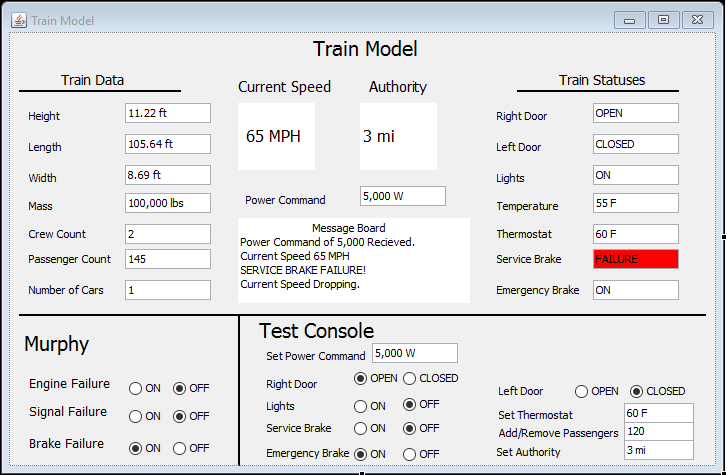
\includegraphics[width=16cm]{trainmodel_gui}
	\caption{Graphical User Interface for the train model}
\end{figure}


\subsection{UI Buttons and actions}
	
	\subsubsection{Train Data}
		\begin{itemize}
			\item Height:  Displays the Height of the train being observed. The height is a constant value obtained from the provided train data sheet.
			\item Length: This value will be displayed to provide the length of the train observed. This value will update as cars are added and removed from the train. From the train data sheet, it was observed that each car was about 106 feet long.
			\item Width:  Displays the width of the train being observed. The width is a constant value obtained from the provided train data sheet.
			\item Mass: This value displays the mass of the train. This will update based on the number of cars attached and number of passengers onboard.
			\item Crew Count: This field displays the number of crew members currently operating the train. This will update based worker schedule as crew members enter and exit.
			\item Passenger Count: This displays the total number of passengers currently on the train. This value will update as passengers embark and disembark.
			\item Number of Cars: This field displays the number of cars currently attached to the train. This will update as cars are added or removed. 
		\end{itemize}

	\subsubsection{Center Console}
		\begin{itemize}
			\item Current Speed:  Displays the current speed of the train. This will be tracked and the value will update periodically as the system runs.
			\item Current Authority:  This value displays the current Authority of the train. This will update accordingly as a new authority is passed to the train from the track.
			\item Power command: This will display the current power command issued to the train model from the train controller. This power will determine the new speed of the train.
			\item Message Board: This section of the console will display event and failure logs of the system periodically as they occur. Notifications such as incoming power commands, current speed and failure statuses will be displayed here
		\end{itemize}

	\subsubsection{Train Statuses}
		\begin{itemize}
			\item Right Door:  Displays the status of the right doors of the train. This will either be shown as “OPEN”, “CLOSED” or “FAILURE”.
			\item Left Door:  Displays the status of the left doors of the train. This will either be shown as “OPEN”, “CLOSED” or “FAILURE”.
			\item Lights:  Displays the status of the interior lights of the train. This will either be shown as “ON”, “OFF” or “FAILURE”.
			\item Temperature: This will display the current temperature inside the train. This will update periodically based on the temperature changes onboard.
			\item Thermostat: This will display the current thermostat settings onboard the train. This will update periodically based on the value set in the train controller.
			\item Service Brake:  Displays the status of the Service brake of the train. This will either be shown as “ON”, “OFF” or “FAILURE”.
			\item Emergency Brake:  Displays the status of the Service brake of the train. This will either be shown as “ON”, “OFF” or “FAILURE”.
	\subsubsection{Murphy Controls}
		\begin{itemize}
			\item Engine Failure: This radio button allows for the user to toggle an engine failure onboard the train.  
			\item Signal Failure: This radio button allows for the user to toggle a signal failure onboard the train. 
			\item Brake Failure: This radio button allows for the user to toggle a failure in the trains service brakes.
		\end{itemize}

	\subsubsection{Test Console}
		\begin{itemize}
			\item Test Console: This console will allow for simulation of the train model without external input from the train controller. This will allow for the user to toggle various inputs that would otherwise be received from the train controller. Changes from these inputs will be displayed in the upper half of the UI.  
			\item Set Power Command: This text field will allow the tester to input a new power command for the train model.
			\item Right Door: This radio button will toggle the right doors between open and closed
			\item Left Door: This radio button will toggle the left doors between open and closed
			\item Lights: This radio button will toggle the interior lights between on and off
			\item Service Brake: This radio button will toggle the service brakes on the train from on and off
			\item Emergency Brake: This radio button will toggle the emergency brakes on the train between on and off
			\item Set thermostat: This text field will allow the test user to input a new thermostat setting for the train.
			\item Add/Remove Passengers: This text field will allow for the test user to input the number of passengers embarking and disembarking at each station. A positive value will add to the current passenger count and a negative value will subtract from the current passenger count
			\item	Set Authority: This text field will allow the test user to set a new authority for the train.
		\end{itemize}


\end{document}